\chapter{Solution}
\label{solution}
\lettrine[lraise=0.1, nindent=0em, slope=-.5em]{\color{Violet}T}{he} Solution chapter is divided int three phases. First, the design phase for planning on learning process. Second, development phase where authoring of learning material being held. Third, the implementation phase the piloting of the course, where each course are run-through with particular students/trainers to get feedback about timing, content and evaluation.



 
\section{Design and Planning of learning process}
The Design phase contains four steps: First, Design learning objectives. Second, design assessments for each objective. Third, choose a course format. Fourth, create an instructional strategy. \citep{website:design_phase_ADDIE}


\subsection{Design of the course content and learning objectives}

In analysis phase the learning outcomes were established. However to design assessments tests and learning material more detailed learning objectives are needed. Therefore each learning outcome are divided into smaller units.

For design an adequate course content two aspects are required, learning objectives and assessment tests. Likewise in software development field the tests should be designed first to ensure creation of consistent learning materials and labs. Therefore all learning objectives are given with evaluation methods and values.  

The terms and vocabulary used in assessment should stay on level the students should know at the end of the lab and derived from learning objectives established in analysis phase.

Because big amount of learning materials, tests and labs only some examples are included into Appendices as Preliminary Tests~\ref{Preliminary Tests}, Preliminary Course~\ref{Preliminary course - dpkg based GNU/Linux}, Protecting Web Application -- \ref{Protecting Web Application Against (D)DOS Attacks},~\ref{Protecting an Insecure Web Application}. However, other materials can be found on course syllabus page composed on section~\ref{Course Syllabus}.


\subsubsection{Pre-requirements courses}

During the analysis of the target group the need for preliminary course was decided to homogenize a knowledge and a skill level of the participants.

The objectives and assessments for preliminary course:
\begin{itemize}
\item Student are able to work in command line using GNU/Linux as working with files, manage software, manage disks and partitions, manage users and groups, configure networks and user login session. Minimal level for pass is to gain more then 50\% one of the tests included in Appendix~\ref{Preliminary Tests} in Table~\ref{tab:preliminary_practical_test}
\item Student are able to explain basic terminology of operating systems (Kernel, GUI, shell, Virtual Memory, Authentication, Authorization, RAM, Cache, puffer, latency, throughput, file system, process, thread, password hash, DAC, MAC, RBAC, command parameter, command flag, file system hierarchy, environment variable). Minimal level to pass is gather more then 51\% of closed book test like in sample in Appendix~\ref{Preliminary Tests}
\item Student are able to configure network in GNU/Linux and explain terms like gateway, netmask, IP address, port, IP alias, DNS servers. Minimal level to pass is configuring network for lab machines.
\item Student is able to read/modify and create simpler BASH, Python and PowerShell scripts. Minimal level of pass is create script with all common language construction in one particular language. Powershell scripting is included because furtherer labs contains also integration labs with Active Directory, SAMBA4, GNU/Linux servers and workstations and Windows workstations.
\end{itemize}

According to previous objectives six practical classes are needed:\footnote{All times are given in academic hours or days which equal 8 academic hours.}
\begin{enumerate}[label=LAB \arabic*.,leftmargin=*]
\item Operating system basics (one day)
\item Basic networking IPv4/IPv6, TCP/IP (one day)
\item GNU/Linux basics (and OpenBSD/FreeBSD basics) (16h) as describbed in Appendix~\ref{Preliminary course - dpkg based GNU/Linux} on page~\pageref{Preliminary course - dpkg based GNU/Linux}
\item Scripting in BASH (2 days)
\item Scripting in Python (1.5 days)
\item Scripting in PowerShell (1.5 days)
\end{enumerate}
After implementing the course exact load is known numbers will be arranged.

\subsubsection{Root Services}
In this particular case term root services are described as \gls{NTP}, \gls{DNS}, \gls{DHCP} service.
After finishing this block student are able to configure root services and use those services in furtherer labs.
The objectives and assessments for Root Services lab:
\begin{itemize}
\item After finishing this lab student is able to install \gls{NTP} service on server and on client computer and configure client to use internal server (pool) and server to use upstream \gls{NTP} service and fall-back services. Minimal level to pass: Services are configured, and student demonstrates debug skills with different tools and user explains basic terms and (pool, stratum, delay , offset, jitter, drift)
\item After finishing this lab student is able to install \gls{DNS} service and configure clients for new server. Minimally, students are able to configure zones, reverse zones, master -- slave replica, forwarding, different type of records (like MX, A, CNAME, TXT for SPF, PTR) and use basic management utilities to reload zone, flush name, flush cache, add records dynamically, freeze and thaw zones). Configured service does recursive quires for one particular subnet and student are able to explain what DNS attacks are used and what is Open Resolver. Student tests \gls{EITC} nameserver and explains what is wrong with that.
\item After finishing this lab student is able to install \gls{DHCP} server and configure hosts using this service. Minimal level for pass: Student installs and configures service what gives networking configuration to client machine from range or using hardware address. Service updates \gls{DNS} records using shared key (Mandatory Access Control must not disabled for pass)
\end{itemize}
According to previous objectives three practical classes are needed:
\begin{enumerate}[label=LAB \arabic*.,leftmargin=*]
  	\item NTP (4h)
  	\item DNS (2.5 days)
  	\item DHCP (one day)
\end{enumerate}

\subsubsection{Web and File services}
Configuring and securing web servers is essential skill required from system administrators. Therefore, web server installation, configuration and hardening are covered with this block. Because instructional goals and learning outcomes also require covering file services topic.

The objectives and assessments for Web and File services:
\begin{itemize}
\item After completing the web and file services block student is able to install web server and web application with database and several virtual hosts and configure \gls{TLS}. Minimal level for passing: Installed web server with two virtual hosts accepting \gls{HTTP} and \gls{HTTPS} connections. Configured IP aliases for \gls{HTTPS} and/or \gls{SNI}.
\item Student is able to use caching technologies to protect web application against simpler \gls{DOS} attacks. Student configures web service and demonstrates that can be easily take offline using simple load generator. Minimal level: Student configures proper caching and demonstrates that web application survives same attack.
\item Student are able to install different application firewalls like \gls{SQL} firewall and web application firewall. Minimal level: Student demonstrates that different types of attacks are possible and successful against particular vulnerable web application. Student installs \gls{SQL} firewall and demonstrates that basic \gls{SQLi} attacks are blocked. Student demonstrates that several web application attacks are still possible (after installing \gls{SQL} firewall reflected \gls{XSS} and possibly stored \gls{XSS}, command injection, \gls{CSRF} are minimum. Student installs application firewall before web application and demonstrates that previously succeeded attacks (at least \gls{XSS}) is stopped.
\item Student is capable to install file server and configure shares, permissions, groups into fileserver. Criteria: Student installs service, configures two shares and group based permissions for share. Student configures client machine to mount shares on demand and on boot.
\end{itemize}


According to previous objectives four practical classes are needed:
\begin{enumerate}[label=LAB \arabic*.,leftmargin=*]
   \item Web server basics - installation and configuring web server (4h)
  	\item Web server security - Protecting Web Application Against (6h)
(D)DOS Attacks
  	\item Web server security - securing vulnerable web application using application firewalls (6h)
  	\item Fileserver (4h)
\end{enumerate}


\subsection{Choosing course format}

For developing e-learning courses the choosing course format is short decision but with big influences to all participants \citep[p.14]{OppeArenduskeskus2010}. 

Common course delivery formats used in e-learning and blended learning (combined form of instruction-led and e-learning) used in \gls{EITC} are: 
\begin{itemize}
\item Asynchronous e-learning - \gls{SIS}, wikis, \gls{LMS}'s, forums, blogs and other collaboration systems.
\item Synchronous e-learning - virtual distance laboratories, remote access for some servers, Skype and other online communications.
\item Instructor-led lessons - practical classes
\item Self-study - homework, reading books and other resources.
\end{itemize}

For this course several methods are used in different cases. First, a self-study are possible because all materials are available from web (except some video materials) in most cases all virtual machines are also publicly downloadable and participants may self-study. Second, combining self-study and instruction-led lessons are used for continuous education groups. Third, a asynchronous e-learning is common and may combined with instruction-led session.

For this e-learning course students can choose combination of asynchronous e-learning, instruction-led lessons (maximum half of the course) or self-study using lecture recordings.

In this particular e-course video lectures are not used but lecture video recordings are available. Also collaboration are preferred and students need to prepare documentation in wiki format and review others work and also give a grade because this method motivates student to produce better documentation and evaluation skills.




\subsection{Instructional strategy}
Instructional strategy for course focuses of guaranteeing learning outcomes by motivation students using proper content and activities planning.


\subsubsection{Pre-instructional activities}
The main goal of pre-instructional activities is motivate the students by explaining to the students why topic started must be covered and what student will be able to do after practical class. Thereafter, present learning objectives and assessment requirements and pre-requirements for the class. However, the minimal requirement level are presented and some students are interested for higher challenges for them extra quests, exercisers are presented as-well.


\subsubsection{Content Presentation}
Most today’s students are bored when receiving only theoretical lecture. For example, 1/2 of students do not have sufficient knowledge to fully understood the topic, and 1/4 of the students know already the aspects given and only 1/4 of the students are in the suitable level.  However, the exact numbers varies but is possible, that similar situation occurs often. Therefore, practical classes and lectures are combined and all taking place in computer classes. Every student should take 15-30 minute long theoretical block followed with practical activities. In case of e-learning students can browse video recordings and do their labs where suitable for them. Moreover, the content presentation should contain a principle author would like to call a \emph{Command Dojo}, where all participants doing the same exercise with same goal with help of the lectures as master with classroom or using screen-cast. The name of the method is derived from \gls{Coding Dojo} in software development~\footnote{A Coding Dojo is a meeting where a bunch of coders get together to work on a programming challenge \url{http://codingdojo.org/cgi-bin/wiki.pl?WhatIsCodingDojo}}.
After completing exercise or running out of time the new goal is given and to demonstrate learned skills the same objective in modifications are given for students and this will assessed by master. The reason behind this solution is simple: Students need good guide to follow and learn, but to show achieved outcomes student needs to configure services without blindly coping and pasting from lab material.

\subsubsection{Learner's feedback and assessment}
After every class, lecture should gather feedback about objectives, theoretical parts, labs and assessments because the course is very intensive and when more then 1/3 students can not follow due some problems then next block will fail for those students because they are linked by topic.
Is also possible that for valuable feedback are sufficient to ask from students how they feel about the course.

\subsubsection{Follow-through activities}
For explaining some situation the active discussions are needed (possible discussion topics are shown in lab materials as questions for the students) as seen in lab material highlighted with blue box with caption Discussion:
\begin{Verbatim}[frame=single,
label=Discussion,framesep=2mm,rulecolor=\color{blue},commandchars=\\\{\}]
Why You can not login into server?
Look at the server console. What is the OOM? What is the OOM killer?
\end{Verbatim}
In case of distance study and self study the discussions should being held using course Skype list. For conclude the discussion the lecturer must give feedback for each discussion topic using same channel or course e-mail list (In \gls{EITC} lecturer can send e-mail messages to all students participating this particular course).



\subsection{Pedagogical view of the e-course}
Different Pedagogical strategies can be used during learning process as \citep{OppeArenduskeskus2010}
\begin{enumerate}
\item problem based learning -- demands analysis approach from student by solving cases based on scenarios derived from real situations
\item collaboration based learning -- based on group-work and cooperation
\item community based learning -- collaboration is community based, helps students to learn from each-other
\end{enumerate}

In case of this e-learning course all three aspects are used and combined.
For labs a problem based learning are used. For documenting a installed service the collaboration based learning are used and course wiki aggregates this information. For review of wiki articles a community based learning are used. However, for continuous education actively used only problem based learning because of intensive nature of the course when no extra time left for homework between contact classes.

\subsection{Planning grading/assessment techniques}
The assessment is used for two proposes: Firstly, ensure achievement of the learning outcomes. Secondly, as a form of the feedback for the student. By planning assessment for an e-learning course the common choises are following~\citep{OppeArenduskeskus2010}
\begin{itemize}
	\item self-assessment
	\item computer assessment
	\item tutor assessment
	\item peer assessment
\end{itemize}

In this course self-assessment are used only for feedback and for entering the course. For example, if system administrator wants to enter the Web and File service course a self-test needed to be done to ensure a presence of the knowledge in level needed by the course. However the computer assessment is easier and less time consuming compared to tutor assessment it insufficient to guarantee the learning outcomes of the student. 

The Computer assessment are used only for guiding and giving feedback to the participant. For example: In case of insecure web application lab the student can execute script that tests application vulnerability with python script performing \gls{SQLi} and test if its filtered by \gls{SQL} firewall or not. The script itself is readable for user and in case of this particular script, it is written by other students as a homework in preliminary scripting course.


The tutor assessment are used to grade the students lab performance and this is time consuming because every student defends their lab solution by reconfiguring services and explaining the architecture and configuration of the solution.

Peer assessment are used in case of documentation grading. Documentation points are given by peer students but tutor assessment are used to grade the graders.

Proper grading are one way to motivate students. Moreover, the competition moment when lab performance are seen by other student gives extra motivation for skilled students but may demotivate weaker ones~\citep{KasakKaur}. In author opinion the competition moment combined with offensive \gls{CTF} type course gives motivation impulse for most of the students. However, this course focused on defence of the systems and the motivation problem is still not solved but possible solution is in implementation.

The idea for motivation system for new course is to implement scoreboard and reward system based on completed and graded labs. For example: Student secures an apache web server using mod security rules the badge are added to student's profile in lab system. Steel coloured badge with apache icon for using application firewall and protecting the system. Silver coloured shield badge when proper report is submitted to "authorities" when, what happened and what student did for mitigation. Gold badge for writing new rules or new scripts or new log parsers to help administrator to deal with the problem. Actually the realization of this system will be a future work in next iteration of the course.

According to \gls{ADDIE} model the next step should be "Choosing technological tools" as audio/video programs and \gls{LMS} system choices, file formats, media authoring programs and choice of collaboration environments~\citep{OppeArenduskeskus2010}. However, this course needs more detailed choices to cover learning objectives and needs for virtualised environment. Therefore, the choices are described in section~\ref{Technical implementation of the e-learning course} as an separate section. 

\section{Technical implementation of the e-learning course}
\label{Technical implementation of the e-learning course}

The general aspects for consideration for choosing technical tools and systems for e-learning course are following~\citep{OppeArenduskeskus2010}:
\begin{itemize}
\item Availability of e-learning course
\item Usability of e-learning course
\item Student motivation
\item Adaptivity
\item Suitability for collaboration
\item Standard compliance
\end{itemize}

Technological tools are needed for following activities: 
\begin{itemize}
\item Sharing study materials
\item Collaboration between students and lectures and communication tools
\item Virtualization environment tools
\item Tools for implementing lab scenarios -- web applications, services, testing programs
\end{itemize}

For sharing study materials the \gls{EITC} wiki~\footnote{\gls{EITC} wiki - \url{https://wiki.itcollege.ee/}} are used because it is public accessible and students can add and edit materials by fixing errors in guides and grading process encourages them to share their knowledge. Study materials are stored in wiki, pdf form. Some tests and temporal assignments are stored into google docs and made available using shared link.

For collaboration also wiki is used to give feedback for student group-works in talk section of the work. All homework are publicly accessible and also reviews. Students even collected all questions asked in defence of the lab and published it. E-mail and Skype are used for usual communication and course forum is implemented in future. Moreover, the configuration files and source files for scripts and learning materials are stored in to public \gls{git} repositories.

Virtualization environments are used for all labs. Several virtualization solutions can be used in this e-learning course. For availability the virtual machines are distributed as Open Virtualization Format (\gls{OVA}) files and are usable in different environments~\footnote{ Distributed Management Task Force (\gls{DMTF}) OVF - \url{http://www.dmtf.org/standards/ovf}}.

Availability of the lab in e-learning form should give access for lab infrastructure from outside of the \gls{EITC} computer classes. Therefore a environment of distance study are implemented in \gls{EITC} and constantly developed to accept needs for new e-learning courses. This course initiated new developments for this environment what is described in next subsection.
Author of this thesis are an architect of the distance study environment and also back- end programmer. In next section the brief overview of the system are given and described new parts of the system developed to support this e-learning course.

\subsection{The Environment of Distance Study}
\label{The Environment of Distance Study}
The motivation to develop environment of distance study was initiated by need to increase amount of practical hands-on work in \gls{EITC}. However, the virtualization was used in computer classes to teach system administration and other subjects the student was not able to continue theirs work after official schedule because virtual machines are stored to local disks of the classroom computer. Moreover, the student was able to use only the same machine like last class and changing classrooms or computers was not possible. However, some students preferred their own laptops for running virtual machines it is hard for labs with several virtual machines because of the requirements for hardware. Moreover, some labs need access to special infrastructure in \gls{EITC} internal LAN, and laptops can not used in this case.

Therefore, the development of the environment of distance study were initiated.

The environment allows students start virtual labs with pre-configured virtual machines. 


\subsubsection{Virtualization Layer}
Siin libvirdist
\subsubsection{Web Application Layer}
Siin Ruby on Rails raamistikust ja veebirakendusest
\subsubsection{Architecture of Distance Laboratory}
Siin räägin üldisest disainist ja allsüsteemidest
\
\begin{figure}[ht]
\centering
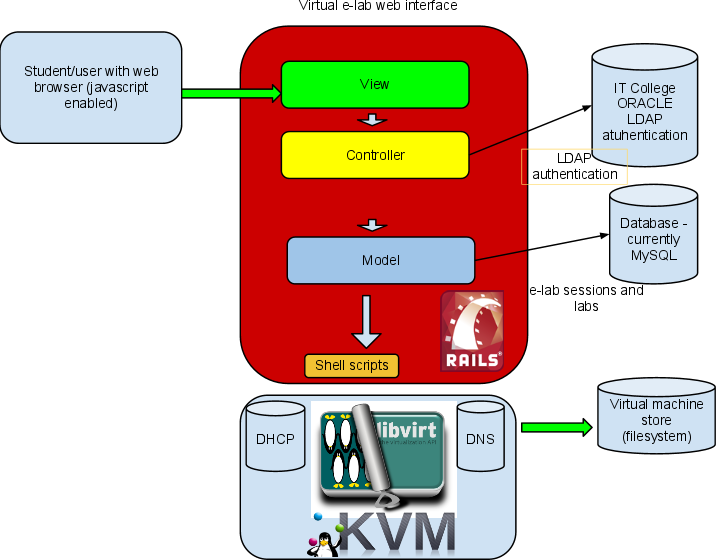
\includegraphics[width=0.8\textwidth]{architecture.png}
\caption{Architecture of Distance Laboratory}
\label{fig:Architecture of Distance Laboratory}
\end{figure}
\

\subsubsection{New developments for distance study environment}

\begin{itemize}
	\item normal traffic generator
	\item malicious traffic generator
	\item availability monitor (for grading)
\end{itemize}

\subsection{Operating Systems used in labs}
Operating systems should use Open Source software for labs exception of PowerShell according to established requirement (in analysis phase)

To maintain diversity and avoid vendor locking a several different operating systems are used in labs. Lab materials are developed using Ubuntu LTS, because of support and popularity, but to get graded the student should choose one different system for defence at least one lab from following list: OpenBSD, FreeBSD, OpenSolaris, Debian GNU/Linux, Fedora, CentOS, Oracle Linux, OpenSuse. Only restriction that chosen system used different packaging from other systems. For example if student chooses Ubuntu to do the \gls{DNS} lab then for \gls{DHCP} should used operating system without debian packaging system.

Labs with offensive parts are done using Kali GNU/Linux distribution but student can also use BackTrack if they want.

The main reason to left choice is open that in labs each student must demonstrate skills and knowledge according to learning objectives and this is more important than knowledge of one system.

\subsection{Choosing software for Root Services lab}
The Root Services labs contains \gls{NTP}, \gls{DNS} and \gls{DHCP} services. However, for fulfilling a learning objectives the software should work on chosen lab platform GNU/Linux Ubuntu Server. For \gls{NTP} common packages are from OpenBSD project and from ISC.

DNS
\subsection{Choosing web server and caching software}

Apache2
NGINX
lighthttp

GreenSQL
Teised tulemüürid


WordPress

MediaWiki

Drupal

Joomla

\subsection{Choosing a vulnerable web application}

The main need for vulnerable web application comes from scenario: Each student installs vulnerable system and must stop basic attacks without reprogramming a web application to reflect usual system administrator's work,  install needed applications and secure them.

Although ready made virtual appliances can be used to install vulnerable web application the
system administrator should be able to install vulnerable application itself to understood a main architecture of web application to choose best protection methods. Therefore chosen application should be free and open source, easily installable, implement at leas stored and reflected \gls{XSS} and several injection type attacks like \gls{SQLi} (usual and blind) and \gls{CSRF}.

\subsubsection{WebGoat}
WebGoat is a free, open source insecure J2EE web application designed to teach web application security lessons.  However the WebGoat is one of the best application for teaching the installation and J2EE requirement is not suitable for system administrators with lesser skills even authors did installation script it hides too many steps valuable for students. 


\subsubsection{Damn Vulnerable Web Application}
The Damn Vulnerable Web Application \gls{DVWA} is web application with several vulnerabilities to be suitable for testing several security vulnerabilities and tools. However, the tool does not implement all \gls{OWASP} top ten attacks the most relevant are presented. The tool is written using PHP/MySQL which are taught for all \gls{EITC} students and known also by system administrators. Moreover the tool is designed for learning and students can choose difficulty level of exploiting \citep{website:dvwa}.

Although the progam is easy to install. Integrated study materials, variable level of  difficulties of vulnerability, the coverage is not best but sufficient.

\subsubsection{NOWASP (Mutillidae)}
NOWASP (Mutillidae) Web Pen-Test Practice Application is a free, open source vulnerable web-application for labs, security enthusiast, classrooms, \gls{CTF}, and vulnerability assessment tool targets. \citep{website:Mutillidae} Although, the tool have video, study materials, good support for \gls{OWASP} top ten the development is relied to one person and community support is thin.
\subsubsection{SQLol}
SQLol is free and open source web application designed to test \gls{SQLi} type injectons and complatible with \gls{MySQL}, gls{PostgreSQL} and uses \gls{PHP}.
cons: only supports \gls{SQLi}
pros: comprehensive  \gls{SQLi} study materials.

 This application was released at at Austin Hackers Association meeting 0x3f by Daniel “unicornFurnace” Crowley of Trustwave Holdings, Inc. – Spider Labs.
Link: https://github.com/SpiderLabs/SQLol



Because of defensive nature on developed course only simple vulnerabilities are needed to demonstrate a problem and all vulnerable applications are suitable for installing. To create diversity all applications what can installed easily can be used in lab. All examples are given using \gls{DVWA} but to get the grade every student should choose another vulnerable application, install it and protect it.

%http://pentestlab.org/10-vulnerable-web-applications-you-can-play-with/ - todo 
Practical Intrusion Analysis book - WAF võrdlus \citep{book:practica_intrusion_analysis}
\gls{CSRF}
Protection using mod\_security
\url{http://blog.spiderlabs.com/2011/01/detecting-malice-with-modsecurity-csrf-attacks.html}

\gls{XSS}
{
\color{red} *Kui avastad, kust on malicious script included siis saab esitada avalduse, et see domeen/virtualhost kinni pandaks...(see võiks olla tulevikus osa laborist.

http://www.dcortesi.com/blog/2009/04/11/twitter-stalkdaily-worm-postmortem/
}


\section{Development of the e-learning course}
The Development phase  (create a sample instruction and evaluate, create course materials - and review, conduct a run-through (a real-time rehearsal of the course) saab tagasisidet ja teada aja, mis on vaja kursuse läbimiseks)

\subsection{Authoring the learning material}
Developing learning material is based on learning objectives. Each learning objective must be covered with learning material and everything else should left out as extra load for student. Therefore in the development phase the authoring of different study materials, assessment tests, audio/video media and integration of all artefacts into consistent body with one reason: ensure that all objectives are met.

Authoring the study materials is one of most time consuming tasks and amount of developed study materials is too big even for appendices. Therefore one sample block - Securing web applications are included in Appendix~\ref{Protecting Web Application Against (D)DOS Attacks} and in Appendix~ \ref{Protecting an Insecure Web Application} 

Developed learning material are publicly available and under (\gls{CC-BY-SA}) license to guarantee maximum impact on field. Therefore is acceptable that people with will and motivation may self-study using this e-learning course. Moreover, the private training companies can use those courses to train target group.

Learning materials, self-tests, course information and other materials are publicly downloadable~\footnote{\href{http://elab.itcollege.ee:8000/cyber-course/}{Course Syllabus (Õpijuhis)}}.


Some never materials are developed using open source revision control system \gls{git} and all changes and commits are publicly available. Moreover, source code of this thesis and labs are available from public \gls{git} repository with \LaTeX  source files and as well other files~\footnote{\href{https://github.com/magavdraakon/margus-thesis.git}{Materials and source code of this thesis}}.


Developed learning material should follow consistent style and present also one example of good documentation practice. For system administrators several howto styles exists. However practical hands-on laboratory instructions are designed that pass through using copy paste is possible but gives one working sample. However, this is not enough to pass lab scenario and student must customize own configuration.

Guiding stile of the lab instruction using style convention: First, all variable parts of the text are clearly differs from other text and command. Second, all commands given by student are highlighted, and variable parts embossed as seen in followed command.


\begin{minted}[frame=lines,framesep=2mm]{bash}
#For changing Out of memory - OOM adjustment score for mysql server
echo "-1000" > /proc/$(pidof mysqld)/oom_score_adj
\end{minted}
%$



Sample sample: Finding a proccess ID of the mysql server proccess.

\begin{minted}[frame=lines,framesep=2mm]{bash}
ps -ef|grep mysqld
\end{minted}
\label{code_sample}
%
\small{
\begin{Verbatim}[frame=single,
label=Command output,framesep=2mm,rulecolor=\color{red},commandchars=\\\{\}]
sudent@opiise:~# ps -ef|grep mysqld
root     11290 10905  0 10:27 pts/6    00:00:00 grep --color=auto mysqld
mysql    \fbox{\color{red}29830}    1  0 Apr25 ?        00:05:47 /usr/sbin/mysqld
\end{Verbatim}
%
}

All study should stored in open formats, like pdf, OpenDocument , MediaWiki markup language, html, utf8 text. Original editable source files for generating pdf, images should be publicly accessible. Moreover, text based materials should stored into version control system like \gls{git} to enable contributing for other lecturers and students as well.



\begin{table}[H]
\centering
\caption{The learning materials}

\begin{tabular}{|p{5cm}|p{3cm}|p{6cm}|}
\hline 
\color{blue}
Name & \color{blue} Comments  & \color{blue} Location \\ 

\hline
  \multicolumn{3}{|c|}{Pre-requirement course} \\
\hline
Operating system basics & & \\
\hline
Basic networking IPv4/IPv6, TCP/IP & & \\

\hline
GNU/Linux basics  & & \\
\hline
Scripting in BASH &  & \\
\hline
Scripting in Python & Co authored with Lauri Võsandi & \\
\hline
Scripting in PowerShell & Author is Heiki Tähis & \\


\hline
\hline
  \multicolumn{3}{|c|}{Root services} \\

\hline 


Lecture - Configuring NTP service & (Estonian 2012), Learning outcome no XXX & \url{http://goo.gl/toRpw} \\ 
\hline 
Practical class - Configuring NTP in Ubuntu  & (Estonian 2012), Learning outcome no XXX , Students improved & \url{https://wiki.itcollege.ee/index.php/NTP_Ubuntus} \\
\hline 
Lecture DNS & & \href{http://enos.itcollege.ee/~mernits/infrastruktuur/Interneti%20domeeninimede%20s%c3%bcsteem%20-%20IT%20infra%20loeng.odp}
{DNS Lecture [OpenDocument]} \\
\hline
Practical class - DNS & Co authored with Katrin Loodus  & \href{https://docs.google.com/document/d/1ZeQpPXdVq1C7RQpxQYR0gBB0OBMYB_0g6aFFxs_-fIA/edit}{Configuring DNS [GoogleDocs] } \\

\hline
\hline
  \multicolumn{3}{|c|}{Web/File Services} \\

\hline 
 & & \\
\hline

\hline
 & & \\
\hline
\hline

\end{tabular} 
\label{table:learning_materials}
\end{table}


\subsection{Course Syllabus}
\label{Course Syllabus}







\subsection{Testing the e-course}

\section{Implementation}

Implementation phase the courses are piloted and feedback from students and other lecturers are gathered, arranging the learning space  and preparing learners for the course~\citep{OppeArenduskeskus2010}.

Author of this thesis piloted each block of the course and collected students feedbacks, notes for improvement ideas and tried to motivate students to behave as active and motivated as possible.
First lab was relatively simple because of simplicity of the topic -- \gls{NTP} compared for example web server lab. However, this was intentional because during this lab the technical details are explained to the students about virtualization environment and roles of lecturer and students in this course. Therefore slow start is important for students to learn environment and organizational aspects of the course. Thereafter, a studies went smoothly for students with proper prerequisite skills and knowledge and hard for others. The main thing learned from implementation: This course is too hard for most of the students but the are motivated to learn the content. However, the preliminary course is mandatory for most of the students and system administrators because small group of students with inadequate level may slow down a whole class.

\begin{table}[h]
\centering
\caption{The evaluation of the implementation stage }
{ \small 
\begin{tabular}{|p{6cm}|p{2cm}|p{5cm}|}
\hline 
\color{blue} Evoluation question & \color{blue} Result [1..4] & \color{blue} Comments and references \\ 
\hline
Students are motivated to be active? 
& 4  &  Active participation of the students are encouraged \\ 
\hline 
Does lecturer give feedback to the students?
& 4 &  Students will get immediate feedback during contact classes, students know that \\ 
\hline 
Did lecturer collect data during the course how to improve course in the future?
& 3 & Data is collected but not yet implemented (will be in next course) \\ 
\hline
Does feedback from student collected?
& 4 & After every course and training feedback are collected. \\ 
\hline 
\end{tabular} 
}
\label{table:implementation_evaluation}
\end{table}

